\section{Face Detection} \label{ch2}

The \textbf{face detection} problem is an instance of the general object detection problem, and its goal is to \textbf{identify and locate human faces in images or videos}, regardless of their position, scale, pose, orientation illumination etc..

\begin{figure}[h!]
		\centering
		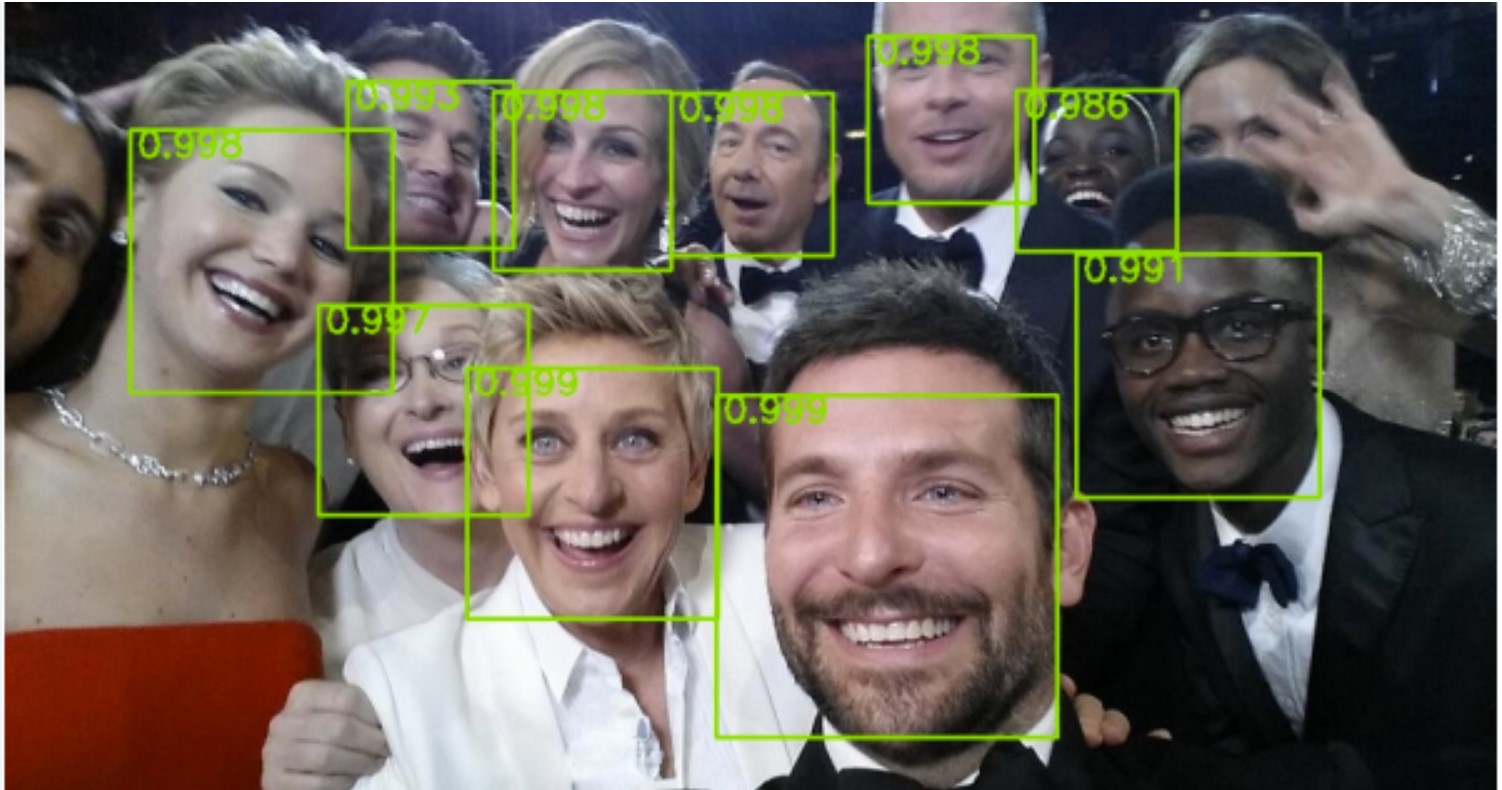
\includegraphics[scale = 0.7]{img/face detection.jpg}
        \caption{Face detection problem}
\end{figure}

If we consider a thumbnail $19$x$19$ face pattern, then there are $256^{231}$ possible combinations of gray values, i.e. $2^{2888}$, which is something like 87 times more than the world population, indicating an extremely high dimensional space! In this sense, the main difficulties of this problem rely on:

\begin{itemize}
    \item the different \textit{scales} of the images;
    \item the different \textit{poses} of the humans in an image;
    \item the problem of \textit{occlusion};
    \item the different \textit{expressions};
    \item \textit{Illumination}.
\end{itemize}

Moreover, there have been examples of images that fooled a \textit{face detection} algorithm.

\begin{figure}[h!]
		\centering
		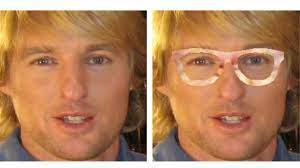
\includegraphics[scale = 0.7]{img/fool.jpeg}
        \caption{Example of image that fools a face detection algorithm}
\end{figure}

\subsection{Related problems}
As we introduced before, the \textit{face detection} problem represents an instance of the more general \textit{object detection} problem, and in turn there exist some related problem to the \textit{face detection}'s one:

\begin{itemize}
    \item \textit{Face localization}, i.e. determine the position of a single face, assuming that the image contains only one face;
    \item \textit{Facial feature extraction}, i.e. detect the presence and locations of features such eyes, nose etc..;
    \item \textit{Face recognition}, i.e. compare an input image, called probe, against a database, called gallery, and report a match. Note that this problem is different from face detection, since in the latter we are not asked to recognize the face: in general, \textit{recognition} is concerned with individual identity, while \textit{detection} with the category of an object;
    \item \textit{Face authentication}, i.e. verify the claim of the identity of an individual in an input image;
    \item \textit{Face tracking}, i.e. continuously estimate the location and possibly the orientation of a face in an image sequence in real time;
    \item \textit{Emotion recognition}, i.e. identifying the affective states (happy, sad, disgusted, etc.) of humans;
\end{itemize}

\subsection{Research issues}
The main issues of \textit{face detection} problem are:

\begin{itemize}
    \item \textbf{Representation}, i.e. how to describe a typical face;
    \item \textbf{Scale}, i.e. how to deal with faces of different scales;
    \item \textbf{Search strategy}, i.e. how to spot the faces;
    \item \textbf{Speed}, i.e. how to speed up the process of spotting;
    \item \textbf{Precision}, i.e. how to locate the faces precisely;
    \item \textbf{Post-processing}, i.e. how to combine detection results.
\end{itemize}

\subsection{Methods}
There exist various methods that are used to address the \textit{face detection} problem, and the most important ones are described below:

\begin{itemize}
    \item \textbf{Knowledge-based methods}: these methods are based on the idea of encoding the human knowledge of what constitutes a typical face (usually the relationships between facial features), and then build a detection algorithm based on these rules. This approach is not related with ML, so it is basically composed of IF-THEN-ELSE;
    \item \textbf{Feature invariant approaches}: in this case the focus is on finding features of a face that are invariant with respect to the pose, the illumination etc.. Still no ML;
    \item \textbf{Template matching methods}: they store several standard patterns to describe the face as a whole or the facial features separately;
    \item \textbf{Appearance-based methods}: these methods exploit the Neural Networks to learn the models (or templates) which capture the representative variability of facial appearance.
\end{itemize}

In the following sections we will provide an analysis of all the methods described above.

\subsubsection{Knowledge-based methods}
As we introduced before, the goal of these methods is to encode the relationships between facial features, i.e. the eyes, the nose etc.., in order to build a detection algorithm based on these rules. In this sense, we can recognize a \textbf{top-down} approach, since the detection is based on a set of human-coded rules. Some examples of these rules are:

\begin{itemize}
    \item the center part of face has uniform intensity values;
    \item the difference between the average intensity values of the center part and the upper part is significant;
    \item a face often appears with two eyes that are symmetric to each other, a nose and a mouth.
\end{itemize}

We analyze two different \textit{knowledge-based methods}: the first one was proposed by \\ \cite{YANG199453}, while the second one by \\ \cite{kotropoulos1994nonlinear}.

\underline{\textbf{Yang and Huang, 1994}}: this algorithm was based on a multi-resolution focus-of-attention approach. In particular,

\begin{itemize}
    \item the \textbf{Level 1}, i.e. the slowest resolution, applied the first rule described above in order to search for candidates;
    \item the \textbf{Level 2} produced a local histogram equalization, in order to correct the image in case of light issues etc.., followed by edge detection;
    \item finally, the \textbf{Level 3} was responsible for searching the eyes and the mouth features for validation.
\end{itemize}

\underline{\textbf{Kotropoloulos and Pitas, 1994}}: the idea of this algorithm was to perform both horizontal and vertical projections of the input image in order to search for candidates. The projections were computed as:

$$
HI(x) = \sum_y I(x,y)
$$

$$
VI(y) = \sum_x I(x,y)
$$

Then, the intersection of these two projections allowed to detect the face. However, it was difficult to detect multiple objects or people in complex background.

In general, the main \textbf{advantage} of this method is that it is quite easy to come up with simple rules to describe the features of a face and their relationships, so for this reason this kind of algorithms are simple to be implemented. Moreover, they obtain really good results for face localization in uncluttered background. On the other hand, the main \textbf{disadvantage} of this approach is that both detailed and general rules to detect faces may find many false positives, and in general it is difficult to extend this approach to detect faces in different poses.

\subsubsection{Feature invariant approaches}
While \textit{knowledge-based methods} follow a top-down approach for detecting faces on an image by following some human-coded rules, the \textit{feature invariant methods} follow a \textbf{bottom-up} approach. Their goal is indeed to detect invariant facial features (for example the eyes, the nose etc..), 
 then to group them into candidates and, finally, to verify them. Since the features are not random, they can be represented as a graph, where the edges represent the relationships between them: in this sense, the \textit{face detection} problem turns into a \textit{graph matching} problem!

 An example of algorithm following this approach was implemented by \\ \cite{leung1995finding}. 
 
 \underline{\textbf{Leung et al, 1995}}: in his solution, he formulated the \textit{face detection} problem as a problem of finding the correct geometric arrangement of facial features, where the facial features were defined by the average responses of multi-scale filters. Finally, the result was given by a graph matching among the candidates to locate faces.

In general, the main \textbf{advantage} of this approach is that, in contrast with the \textit{knowledge-based methods}, in this case the features are invariant to the pose and the orientation changes. On the other hand, two \textbf{disadvantages} of this method are that it is difficult to locate facial features due to several corruption (for example, illumination, noise etc..), and to detect features in complex backgrounds.

\subsubsection{Template matching models}
This approach is similar to the previous one, since its goal is to store one or more hand-coded templates and to use the correlation between the templates and the image in order to locate faces. The templates can be either predefined, i.e. they are based on edges or regions, or deformable, i.e. they are based on facial contours, so they adapt to different faces. Pictures \ref{predefined} and \ref{deformalble} represents, respectively, an example of predefined and deformable templates: as we can see, in both cases the goal of the algorithm is to find some points in the image that match with the template.

\begin{figure}[h!]
		\centering
		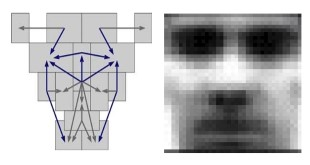
\includegraphics[scale = 1.5]{img/predefined.jpg}
        \label{predefined}
        \caption{Example of predefined template}
\end{figure}

\begin{figure}[h!]
		\centering
		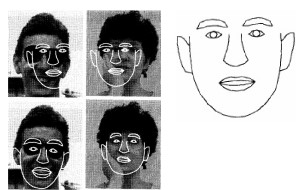
\includegraphics[scale = 1.5]{img/deformable.jpg}
        \label{deformalble}
        \caption{Example of deformable template}
\end{figure}

In general, these algorithms are simple, but on the other hand they need the templates to be initialized near the face images, and it is difficult to enumerate all the possible templates for different poses (similarly to knowledge-based methods)

\subsubsection{Appearance-based methods}
The last family of methods we analyze are the \textit{appearance-based methods}, which are the only ones characterized by a ML (or data driven) approach. The general idea of these algorithms is to:

\begin{enumerate}
    \item Collect a large set of (resized) face and non-face images and to train a binary classifier to discriminate them;
    \item Given a test image, they detect faces by applying the trained classifier at each position and scale of the image
\end{enumerate}

Note that the second phase ensures that the algorithms are invariant to different positions and scales. We will analyze three different algorithms: the first one was introduced by \cite{sung1998example}, the second one by \\ \cite{rowley1998neural}, while the third one by \cite{viola2001rapid}.

\underline{\textbf{Sung and Poggio, 1994}}: the main idea of this algorithm is to exploit the sliding window approach. In particular, the sliding window moves across the image running a classifier in order to detect if the portion contains an image or not. Note that this technique is repeated for different sizes of the image, in order to make it invariant to scale. Moreover, as mentioned before, the \textit{appearance-based methods} exploit the functioning of the Neural Networks, and in this case the \textit{back-propagation}  technique was exploited. Overall, the algorithm was composed of several phases, which are described below, while Picture \ref{poggio_overview} represents an overview of the algorithm.

\begin{figure}[h!]
		\centering
		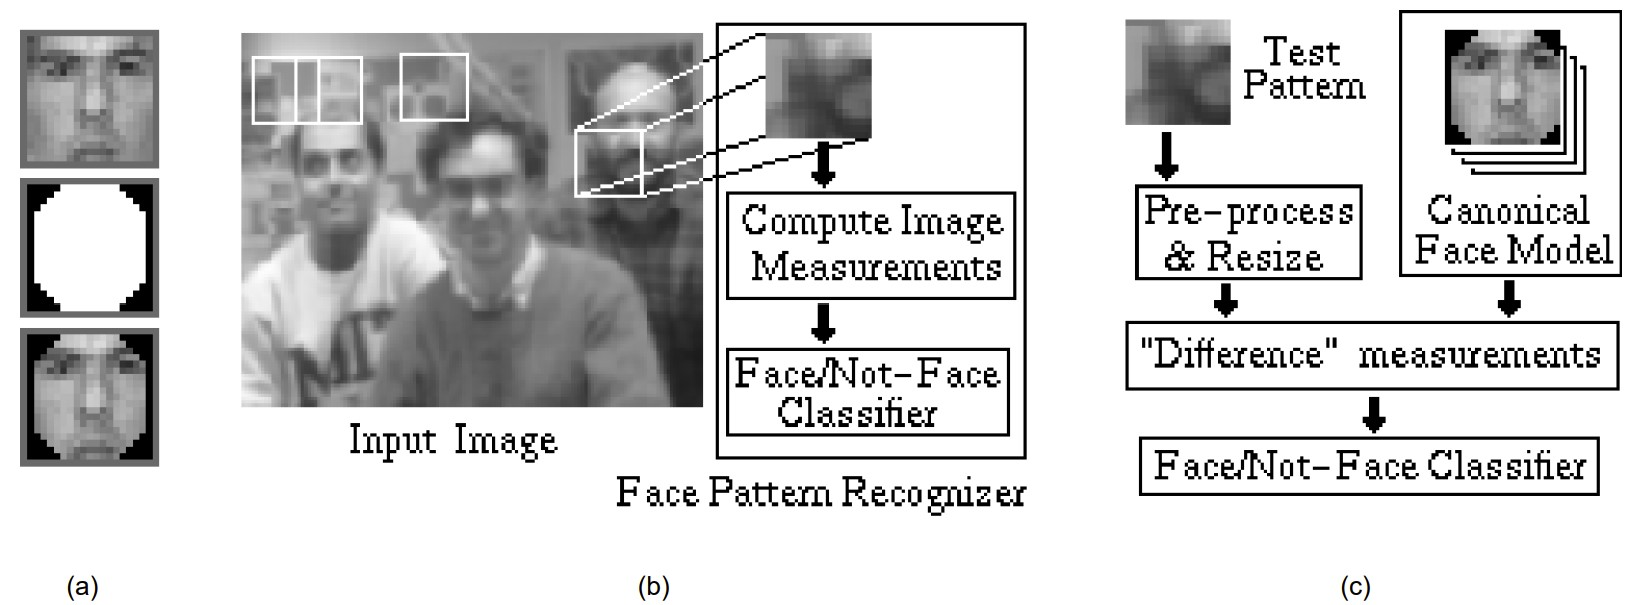
\includegraphics[scale = 0.7]{img/poggio_overwiew.jpg}
        \label{poggio_overview}
        \caption{Overview of the algorithm}
\end{figure}

\begin{enumerate}
    \item \textbf{Pre-processing phase}: in this phase the input image is "cleaned" in the following steps:
    \begin{itemize}
        \item \textbf{Resizing}, i.e. all the image patterns are resized to 19x19 pixels;
        \item \textbf{Masking}, which reduces the unwanted background noise in a face pattern. This is done by using an oval mask, and not a rectangular one, exploiting the fact that the face in the image does not fill the corner of a rectangular mask;
        \item \textbf{Illumination gradient correction}, which finds the best fit brightness plane and then subtract from it to reduce heavy shadows caused by extreme lightning angles. This step is done for solving face detection problem for images with shadows;
        \item \textbf{Histogram equalization}, which compensates the imaging effects due to changes in illumination and different camera input gains.
    \end{itemize}
    
    \item \textbf{Modeling the distribution of "face" and "non-face" patterns}: now the goal is to classify each portion of the image, and this is done by building a training set composed by both positive examples and negative examples (always 19x19 images). Then the idea was to consider these examples as points, and to cluster these points into \textbf{6 different clusters} by using $K Means$ algorithms, in order to group faces with similar expression (they estimated in 6 the number of different expression of a human face). Each cluster is modeled by a multi-dimensional Gaussian with a centroid and a covariance matrix, and each Gaussian covariance is approximated with a subspace, i.e. by using the largest eigenvectors. A visual representation of this phase is provided in Picture \ref{poggio_clusters}.

    \begin{figure}[h!]
		\centering
		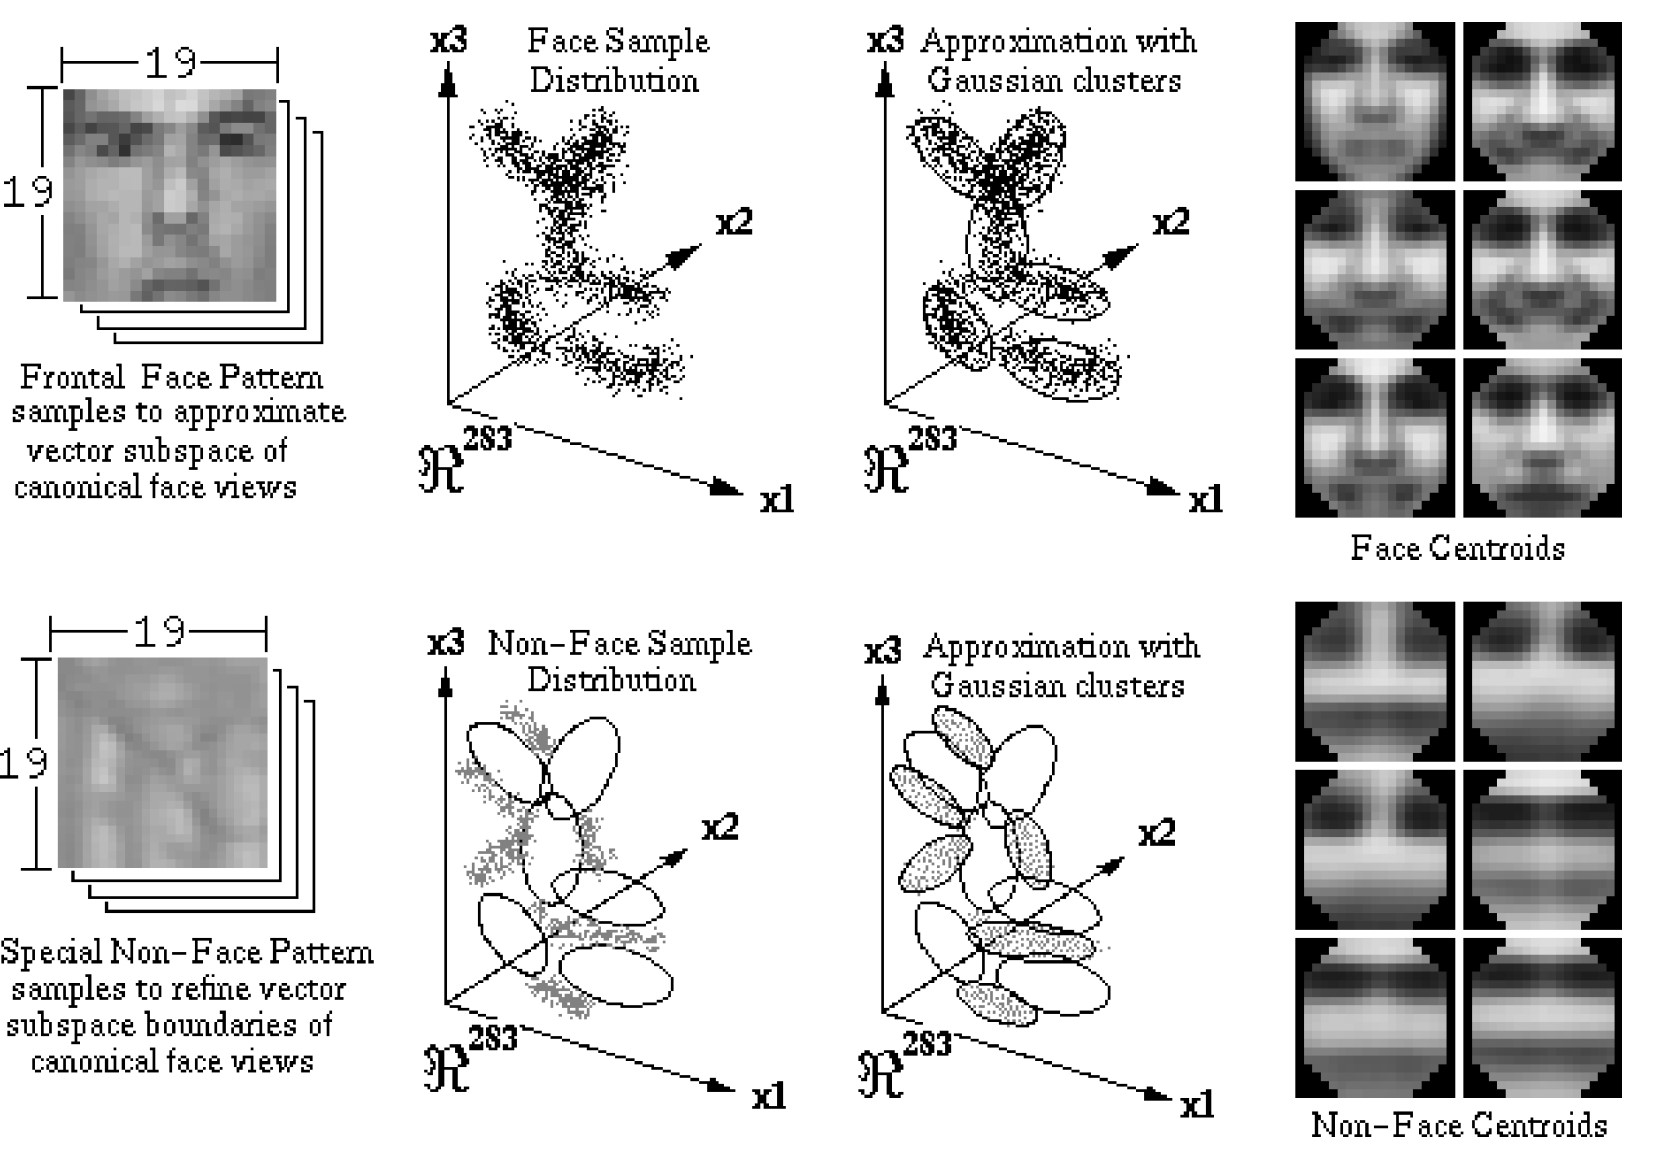
\includegraphics[scale = 0.7]{img/poggio_clusters.jpg}
        \label{poggio_clusters}
        \caption{Second phase of the algorithm}
    \end{figure}

    \item \textbf{Matching patterns with the model}: to detect faces in an input image, the system matches window patterns at different image locations and scales against the distribution-based face model. Before each match, the system first applies the preprocessing operations to the current window pattern. Each match returns a \textbf{set of “difference” measurements} which is fed to a trained classifier that determines whether or not the current window pattern is a frontal face view. More specifically, each set of measurements is a \textbf{feature vector of 12 distances} between the normalized input window pattern and the model’s 12 cluster centroids in our multidimensional image vector space, as represented in Picture \ref{poggio_measurements}. 

    \begin{figure}[h!]
		\centering
		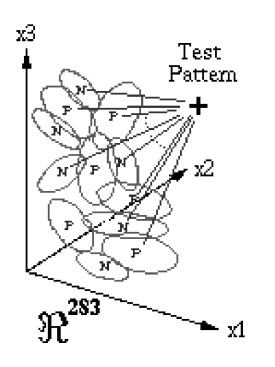
\includegraphics[scale = 1.2]{img/poggio_measurements.jpg}
        \label{poggio_measurements}
        \caption{Set of "difference" measurements}
    \end{figure}

    Moreover, each of the 12 distances is composed of two parts:

    \begin{itemize}
        \item the \textit{within subspace distance} $D_1$, which is represented by the Mahalanobis distance between the projected sample and the cluster centroid;
        \item the \textit{distance to the subspace} $D_2$, which is represented by the distance between the sample and the subspace.
    \end{itemize}

    A visual representation of $D_1$ and $D_2$ is provided in Picture \ref{poggio_distance}.

    \begin{figure}[h!]
		\centering
		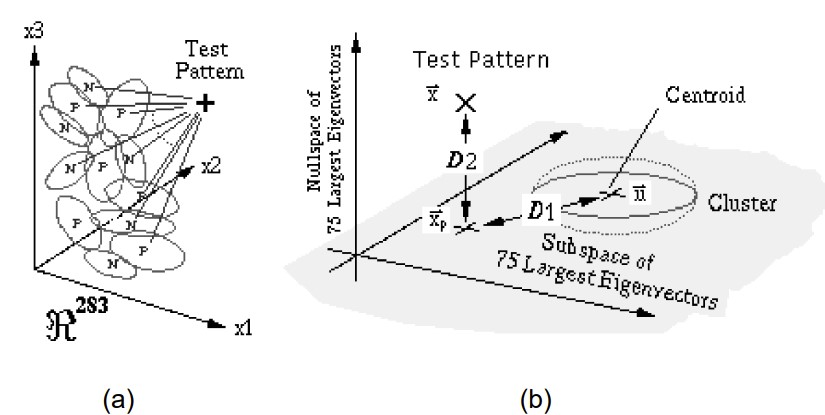
\includegraphics[scale = 1.2]{img/poggio_distance.jpg}
        \label{poggio_distance}
        \caption{Visual representation of $D_1$ and $D_2$}
    \end{figure}

    \item \textbf{The classifier}: the final phase of the algorithms is the classification phase. A \textbf{Multi-layer Neural Network} is used to identify "face" windows patterns from "non face" patterns by using the feature vector of 12 distances derived from the previous phase. The network has:

    \begin{itemize}
        \item 12 pairs of input units, each of which representing a pair $(D_1,D_2)$ of distances;
        \item 24 hidden units (it was proved that this number does not significantly affect the network's performance);
        \item 1 output unit ("face" or "non face").
    \end{itemize}

    During classification, the net is given a vector of the current test pattern’s distance measurements to the 12 cluster centroids: the output unit returns a 1 if the input distance vector arises from a “face” pattern, and a 0 otherwise. The net was trained on feature distance vectors from a database of 47,316 window patterns containing 4,150 positive examples of “face” patterns with a standard \textbf{back-propagation learning algorithm} until the output error stabilizes at a very small value.

\end{enumerate}

A crucial aspect of this algorithm is that the feature vector was not chosen from the image, but it was built by using a set of distances from the test patterns: in this sense, the Neural Network worked as a Nearest Neighbor classifier. Another important issue of this method was the \textbf{generation of the training set}. As we described above, the training set was composed by both positive and negative examples: for "face" patterns the selection was quite simple, because the simply collected all the possible views of human faces. However, since the collection of "face" patterns was not so large, their idea was to increase it by creating some \textbf{virtual examples}, each of which was derived by randomly mirror, rotate, translate and scale the original "face" examples. This technique is called nowadays \textbf{data augmentation}. Picture \ref{poggio_virtual} shows some virtual examples.

\begin{figure}[h!]
		\centering
		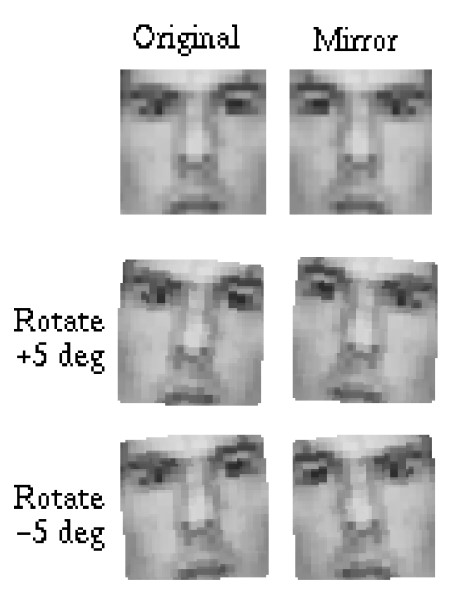
\includegraphics[scale = 1.0]{img/poggio_virtual_examples.jpg}
        \label{poggio_virtual}
        \caption{Virtual examples}
\end{figure}

For “non face” patterns, the task is more tricky. In essence, every square non-face window pattern of any size in any image is a valid training example. Clearly, our set of “non face” patterns can grow intractably large if we are to include all possible “non face” patterns in the training set. To constrain the number of “non face” examples in the training set, they used the following \textbf{bootstrap} strategy that incrementally selects only those “non face” patterns with high utility value with the following steps:

\begin{enumerate}
    \item Start with a random small set of "non face" examples in the training set;
    \item Train the Neural Network classifier with the current training set;
    \item Run the learned face detector on a sequence of random images;
    \item Collect all the "non face" patterns that the current detector wrongly classified as faces, i.e. the false positives;
    \item Add these "non faces" patterns to the training set;
    \item Repeat from 2 until satisfied.
\end{enumerate}

Note that this technique leads to two important consequences: the first one is that it provides a simple method to build "non faces" patterns, and the second one is that the training set is enlarged with examples that steer the classifier away from its current mistakes.

Finally, one last feature of this algorithm is that in order to be invariant to different scales, the input images were downsampled by a certain scaling factor. Picture \ref{poggio_results} shows a result of the algorithm.

\begin{figure}[h!]
		\centering
		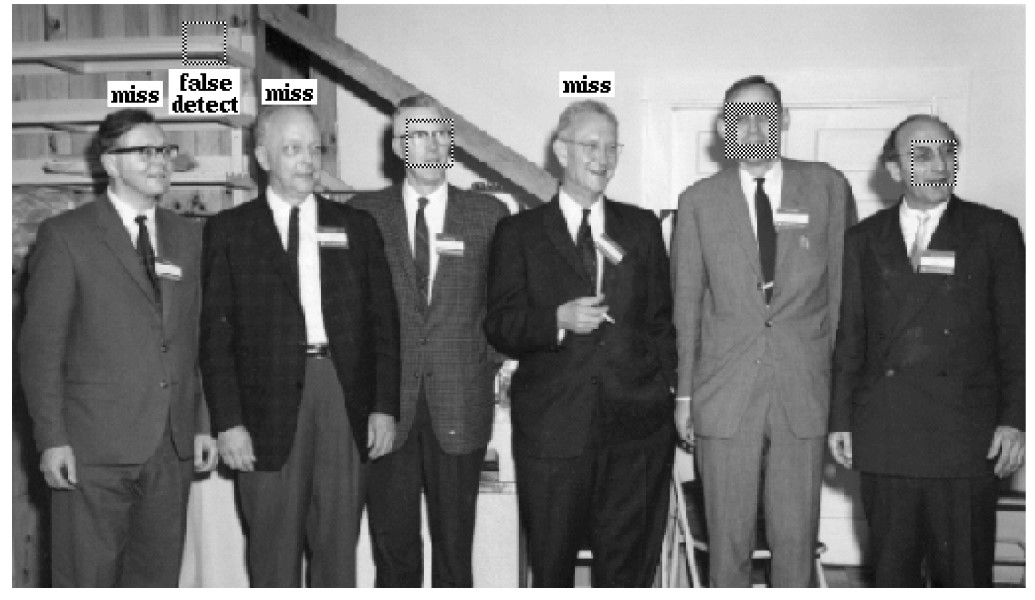
\includegraphics[scale = 1.0]{img/poggio_results.jpg}
        \label{poggio_results}
        \caption{Results of the algorithm}
\end{figure}

\underline{\textbf{Rowley-Baluja-Kanade (1996)}}: this algorithm is much similar to what we do nowadays, and the main difference with the previous one relies on the way in which the Neural Network is used, while the pre-processing and the other phases are quite similar. Picture \ref{rowley_overview} represents an overview of the algorithm.

\begin{figure}[h!]
		\centering
		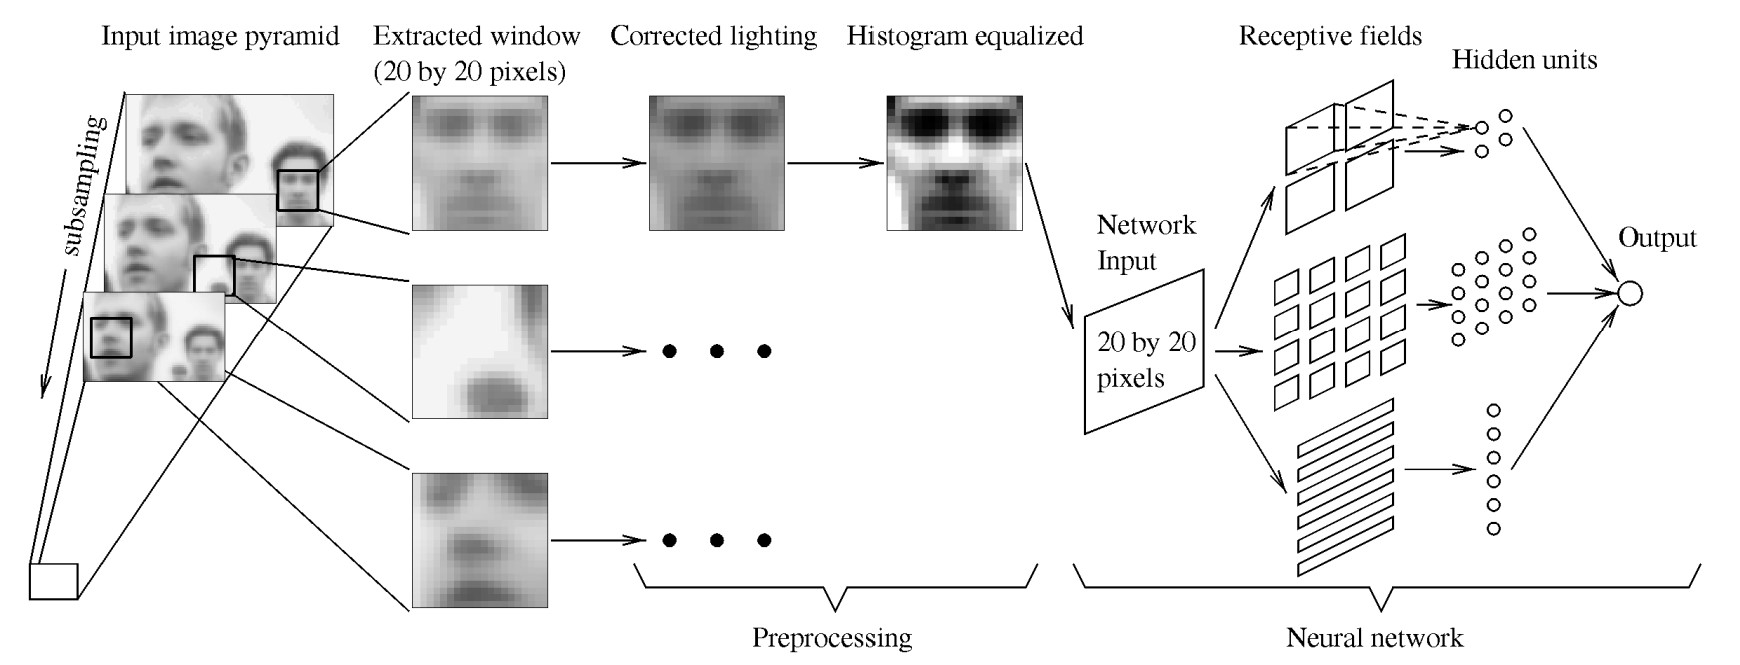
\includegraphics[scale = 0.7]{img/rowley_overview.jpg}
        \label{rowley_overview}
        \caption{Overview of the algorithm}
\end{figure}

As we can see, the pre-processing phase is very similar to the previous algorithm, with the only difference with the size of the patterns, which is now 20x20 (the previous one was 19x19). As we said before, the main difference relies in the \textbf{Neural Network}: in this case the features were extracted directly from the image, and they exploited the concept of \textbf{receptive field} of a neuron. While in a standard Neural Network, each neuron receives in input all the outputs of the neurons in the previous layer, in a Neural Network with receptive fields, each hidden unit receives in input the outputs of a subset of neurons of the previous layer, as showed in Picture \ref{receptive}. 

\begin{figure}[h!]
		\centering
		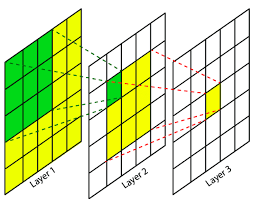
\includegraphics[scale = 0.5]{img/receptive_field.png}
        \label{receptive}
        \caption{Representation of the functioning of the receptive field of a neuron}
\end{figure}

In this sense, in this algorithm the input patch was splitted in several sub-regions, each of which was "controlled" by different neurons. The size of the receptive fields of the hidden unit were different, in order to detect local features that could be important for the problem of face detection. In particular, the hidden units with horizontal receptive fields were able to detect such features as mouths or pairs of eyes, while the hidden units with square receptive fields were able to detect features such as individual eyes, the nose, or corners of the mouth. 

The overall performances of this algorithm were better than Sung and Poggio, and in general their results were astonishing at that time. In Picture \ref{rowley_results} we provide an example of result of this algorithm.

\begin{figure}[h!]
		\centering
		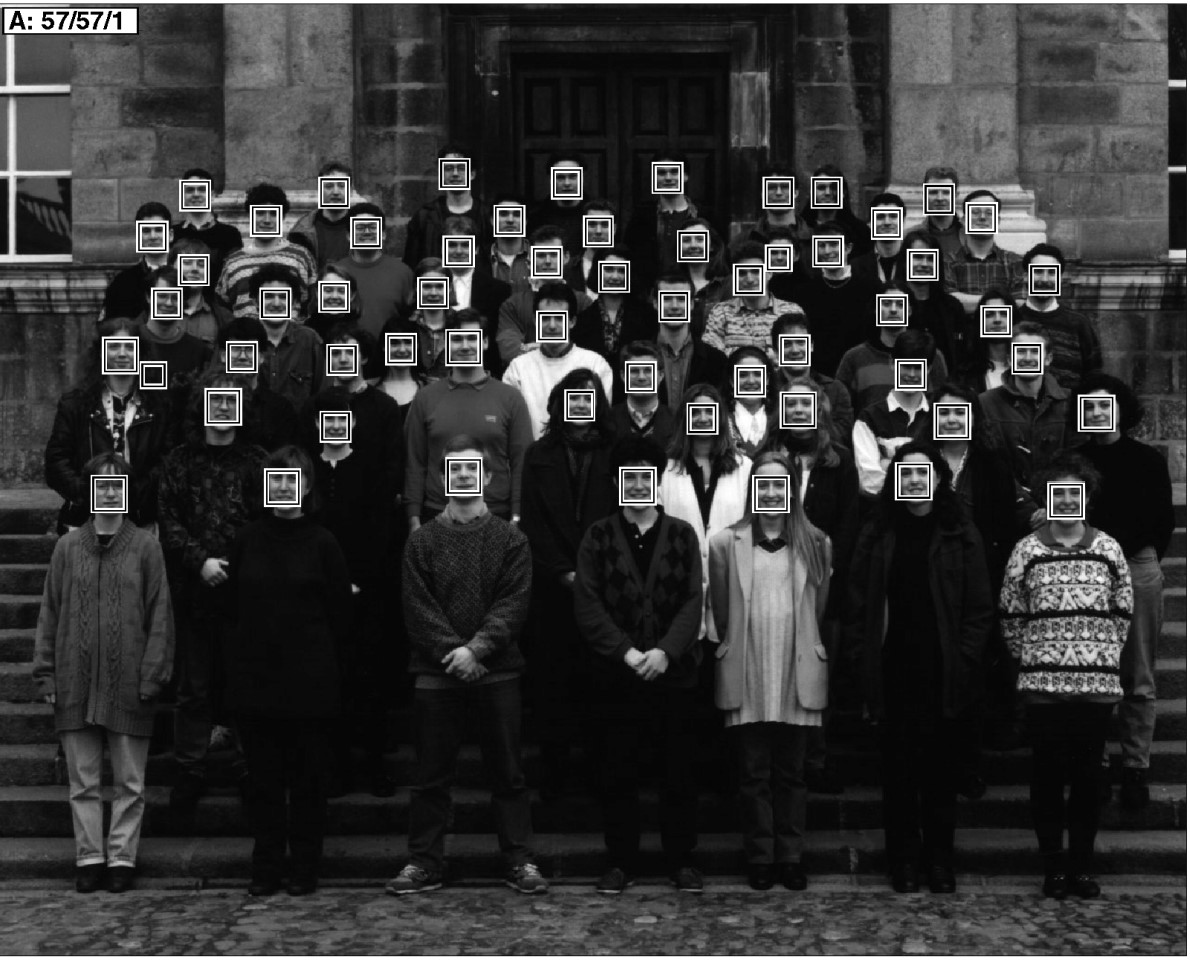
\includegraphics[scale = 0.6]{img/rowley_results.jpg}
        \label{rowley_results}
        \caption{Results of the algorithm}
\end{figure}

However, in 1998 the same authors provided a new version of the algorithm \\ (\cite{rowley1998rotation}) which was able to detect \textbf{rotated faces}. The idea for solving this new problem was the following one: before feeding the face detector, they built a Neural Network, called \textit{Router Network} which was trained to estimate the rotation angle of the input window. If the window contained a face, the the \textit{Router} returned the angle of the face and the face was rotated back to upright frontal position, otherwise it returned a meaningless angle. Then, the de-rotated window was applied to the face detector, which was previously trained for upright frontal faces. Picture \ref{rowley_rotated} represents an overview of this second version of the algorithm.

\begin{figure}[h!]
		\centering
		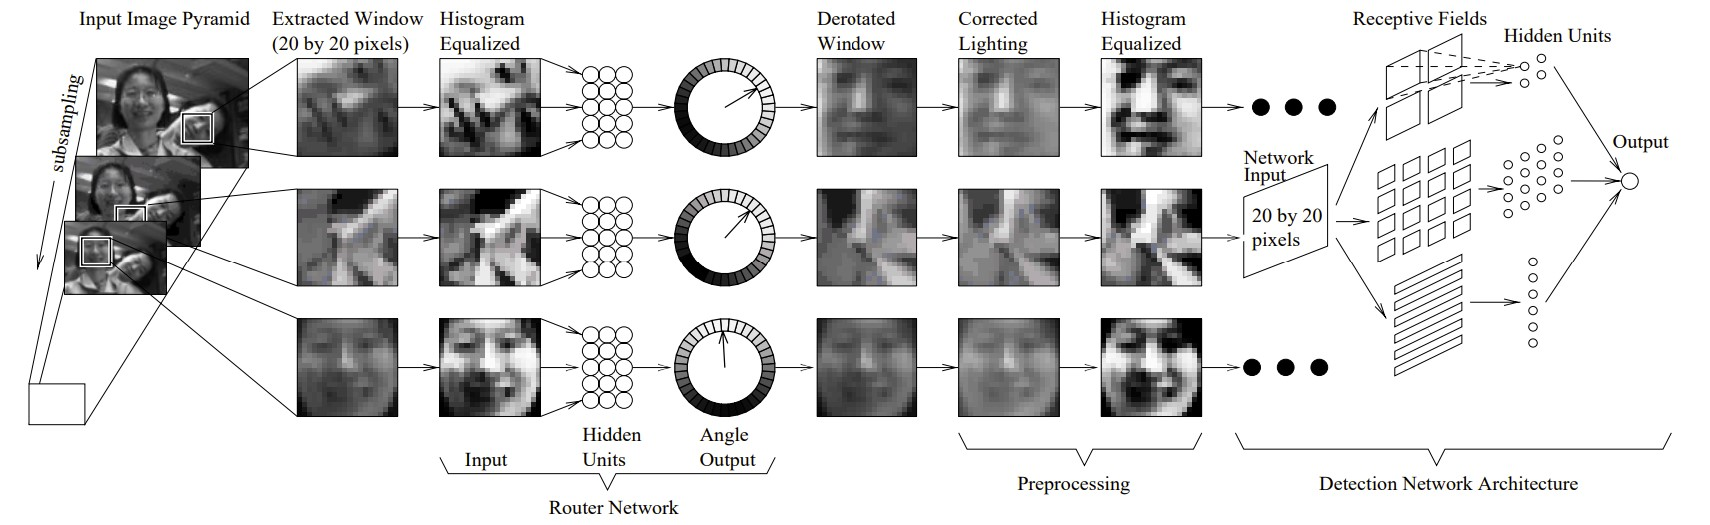
\includegraphics[scale = 0.8]{img/rowley_overview_rotated.jpg}
        \label{rowley_rotated}
        \caption{Overview of the new version}
\end{figure}

In order to implement these operations, the training set for the \textit{Router Network} was built by exploiting the so-called \textbf{self learning} technique, which avoids to manually label the whole training set. The value of the rotation angle for each image was not manually added, but it was retrieved by rotating the original upright image by a certain value, which therefore was added in the training set. 

Despite being much more accurate that Sung and Poggio, this algorithm had still some problems with the accuracy, and, especially, it had unacceptable CPU times.

\underline{\textbf{Viola and Jones, 2001}}: this algorithm represented the first real-time face detector, and for this reason it was implemented in real systems for a long time. It was characterized by a slow training phase, while the detection phase was very fast; in general, the three main contributions of this work were:

\begin{enumerate}
    \item A new image representation called \textbf{integral image}, which allows the features used by the detector to be computed in a very fast way;
    \item A learning algorithm, based on \textit{AdaBoost}, for feature selection: it selects a small number of critical visual features from a larger set and yields extremely efficient classifiers;
    \item A method, called \textbf{attentional cascade}, for fast rejection of non face windows. The idea was to use sliding windows, but without wasting any time in a non face portion of the image.
\end{enumerate}

Now we focus on each of the three contributions. In general, the object detector was based on very \textbf{simple features}: they used \textit{two-rectangle features}, \textit{three-rectangle features} and \textit{four-rectangle features}, as represented in Picture \ref{viola_features}.

\begin{figure}[h!]
		\centering
		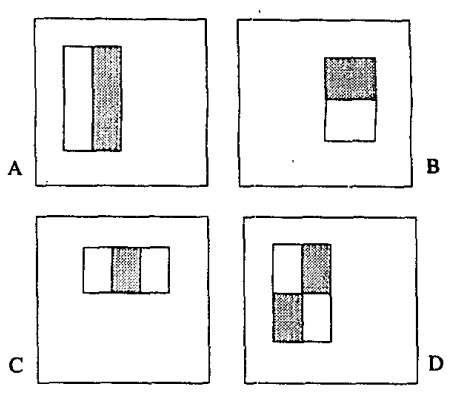
\includegraphics[scale = 1.2]{img/viola_features.jpg}
        \label{viola_features}
        \caption{Rectangular features}
\end{figure}

Each of the features computed the sum of the values in the white area subtracted by the sum of the values in the black area. In this way, the value of the feature was maximum if all the relevant pixels of the underlying portion of the image were positioned under the white area of the rectangle. An example is represented in Picture \ref{viola_features_2}.

\begin{figure}[h!]
		\centering
		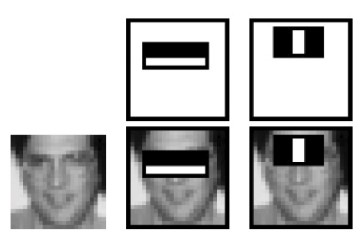
\includegraphics[scale = 1.2]{img/viola_features2.jpg}
        \label{viola_features_2}
        \caption{Features and an image}
\end{figure}

Moreover, the rectangle features can be computed very quickly using an intermediate representation of the image that is called \textbf{integral image}. The \textit{integral image} computes a value at each pixel $(x,y)$ as the sum of the pixel values above and to the left of $(x,y)$ inclusive, i.e.

$$
ii(x,y) = \sum_{x' \leq x, y' \leq y} i(x',y')
$$
, where $i(x',y')$ corresponds to the original image. An important property of the \textit{integral image} is that it can be computed in a single pass over the image, i.e. in linear time, by considering the following pair of recurrences:

$$
s(x,y) = s(x-1,y) + i(x,y)
$$

$$
ii(x,y) = ii(x,y-1) + s(x,y)
$$
, where $s(x,y)$ represents the cumulative sum of the row values.
In this sense, we can exploit this important property in order to compute in linear time the sum of the values of the rectangular features. For example, if A,B,C and D are the values of the \textit{integral image} at the corners of a rectangle, then the sum of the original image values in the rectangle is given by A-B-C+D. As we can see, only three additions are required for any size of the rectangle, which make the feature extraction a very fast operation. Notice that for a 24x24 detection region, which was the region used in the model, the number of possible rectangle features is around 180,000.

Then, the second important innovation of the algorithm was about the \textbf{learning algorithm} adopted both for the feature selection phase and to train the classifier, which was based on the \textbf{ensemble approach}. While in a standard ML pipeline a single complex learning algorithm is trained with the training set and tested with the test set, in the \textit{ensemble approach} a family of weak algorithms is trained, and the prediction is taken from the majority vote or the average of the predictions of all the weak algorithms. Note that a "weak learner" needs only to do better than chance, i.e. better than a model that predicts by tossing a coin. The functioning of this approach is represented in Picture \ref{ensemble}.

\begin{figure}[h!]
		\centering
		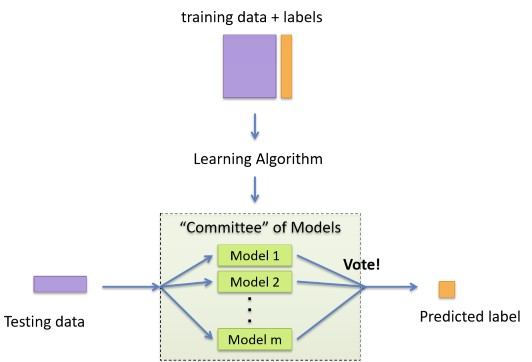
\includegraphics[scale = 1.4]{img/enseble.jpg}
        \label{ensemble}
        \caption{Functioning of the ensemble methods approach}
\end{figure}

One example of algorithms exploiting this idea of the \textit{ensemble methods} is the \textbf{Boosting} algorithm: in this case each weak model is trained sequentially, and the instances that are misclassified by a model are given more weight, i.e. more attention, so that the following model focuses more on classifying correctly those instances.

\begin{figure}[h!]
		\centering
		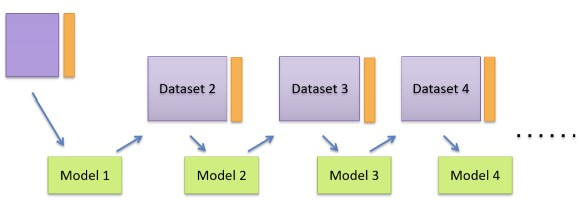
\includegraphics[scale = 1.4]{img/boosting.jpg}
        \label{boosting}
        \caption{Boosting algorithm}
\end{figure}

In particular, the \textit{Boosting} algorithm can be summarized as follows:

\begin{enumerate}
    \item Initially, all the weights of the training set are equal;
    \item In each boosting round, the weak learner that achieves the lowest weighted error in chosen, and the weights of the training examples that are misclassified by this learner are risen;
    \item The final classifier is computed as a linear combination of all weak learners, where the weight of each learner is directly proportional to its accuracy.
\end{enumerate}

The exact formulas for re-weighting and combine the weak learners depend on the particular boosting scheme (e.g. \textit{AdaBoost}). 

As we said before, even though each of the rectangular feature could be computed very efficiently by exploiting the \textit{integral image} representation, computing the complete set of 180,000 features was prohibitively expensive. Their hypothesis was that a very small number of these features could be combined to form an effective classifier, so the \textit{feature extraction} phase was implemented using the \textit{ensemble approach} define above. More specifically, for each feature, the weak learner determines the optimal threshold classification function, such that the minimum number of examples are misclassified. From a mathematical point of view, the learner is defined as:

$$
h_j(x) = \begin{cases}
	1 \qquad \text{if } p_jf_j(x) < p_j\theta_j\\
	0 \qquad \text{otherwise}
	\end{cases}
$$
, where:

\begin{itemize}
    \item $x$ is a 24x24 window of the image;
    \item $p_j$ is a parity bit, i.e. it is equal to 1 if we impose the feature to be greater than the threshold, -1 otherwise;
    \item $f_j(x)$ is the response of the rectangle feature, computed using the \textit{integral image};
    \item $\theta_j$ is the thershold.
\end{itemize}

Finally, Picture \ref{adaboost} represents the \textit{AdaBoost} algorithm which was implemented for both feature selection and training the classifier.

\begin{figure}[h!]
		\centering
		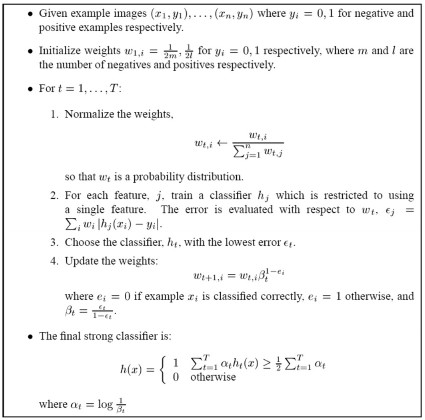
\includegraphics[scale = 1.8]{img/adaboost.jpg}
        \label{adaboost}
        \caption{AdaBoost algorithm}
\end{figure}

Some notes:

\begin{itemize}
    \item The training set is composed of both positive and negative examples;
    \item The weights are initialized uniformly;
    \item Point 2. computes the error of the learner w.r.t. the feature $j$: notice that $|h_j(x_i) - y_i|$ represents the actual error of the learner, while $w_i$ represents the weight of the example;
    \item Point 4. updates the weights of the examples: notice that $\beta_t < 1$, so if the example is correctly classified, then its weight is reduced, otherwise it remains the same. However, since the weights are normalized, this reduction will lead to an increase of the weights of the misclassified examples.
\end{itemize}

The first feature that was selected seemed to focus on the property that the region of the eyes is often darker than the region of the nose and cheeks , while the second selected feature relied on the property that the eyes are darker than the bridge of the nose. This feature combination could yield almost 100\% detection rate and 50\% false positive rate. Moreover, it was proved that a 200-features classifier could yield to a 95\% detection rate with a false positive rate of 1 in 14084; however, adding features to the classifier directly increases the computation time.

The last crucial idea developed in this model was the method of \textbf{attentional cascade}, whose goal was to construct a cascade of classifiers which achieves increased detection performance while radically reducing computation time. The key idea is that smaller, and therefore more efficient, boosted classifiers can be constructed in order to reject many of the negative sub-windows while detecting almost all positive instances. Simpler classifiers are used to reject the majority of sub-windows before more complex classifiers are called upon to achieve low false positive rates. A visual representation of this method is provided in Picture \ref{cascade}.

\begin{figure}[h!]
		\centering
		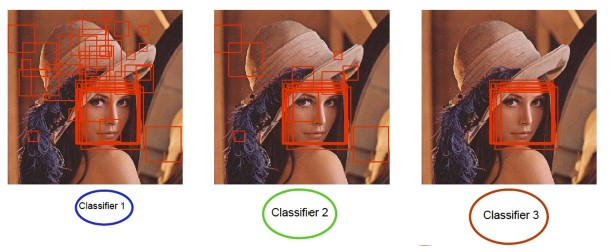
\includegraphics[scale = 1.8]{img/cascade.jpg}
        \label{cascade}
        \caption{Attentional cascade}
\end{figure}

 As we can see, the first classifier sees all the possible sub-windows, but a negative outcome at any point leads to the immediate rejection of the sub-window, which is therefore not considered by the following, a more complex classifier. In the case of the \textit{attentional cascade} method, both the detection rate and the false positive rate are computed by multiplying the respective rates of the individual stages: in general, it was proved that a detection rate of $0.9$ and a false positive rate of $10^{-6}$ can be achieved by a 10-stage cascade if each stage has a detection rate of $0.99$ and a false positive rate of $0.30$. Two possible problems about the \textit{attentional cascade} approach can be either that a classifier rejects a sub-window in which there's a face or that several detections are found for a single face. In particular, the second issue is shared among all the appearance-based methods we discussed, and it can be solved by applying the \textit{non-maximum suppression} method, which is implemented as follows:

 \begin{itemize}
     \item The set of detections are first partitioned into disjoint subsets: two detections are in the same subset if their regions overlap;
     \item Each partition yields a single final detection, whose corners are the average of the corners of all detections in the subset.
 \end{itemize}

A visual result of the application of the \textit{non-maximum suppression} method is provided in Picture \ref{nms}.

\begin{figure}[h!]
		\centering
		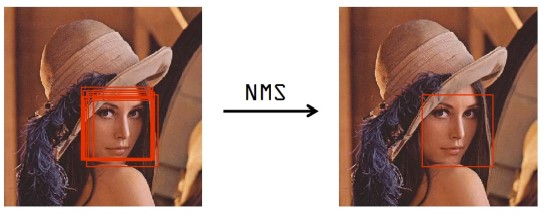
\includegraphics[scale = 1.8]{img/nms.jpg}
        \label{nms}
        \caption{Result of non-maximum suppression process}
\end{figure}

The \textit{Viola and Jones} algorithm was trained with 4,916 hand labeled faces and 10,000 non faces, containing many variations (illumination, pose etc..). The training phase took several weeks, and the final detector contained 38 layers for a total of 6,061 features. The test time was 15 times faster that \textit{Rowley-Baluja-Kanade}.
